\chapter{Context Discovery Framework}

\section{Pruning Search Spaces with CueNet}

Automatic media annotation algorithms essentially assign one or more labels from a search space to a given input image. Figure \ref{fig:with-without-cuenet} shows the various approaches of constructing such a search space for such an algorithm. The traditional approach is shown in \ref{fig:with-without-cuenet}(a). These spaces were limited to a set of labels chosen by an expert, with no way of pruning the search space in case it got very large. The focus was instead on extracting the best features from images, to obtain high overall classification accuracy\cite{turk1991eigenfaces}.

\begin{figure}[t]
\centering
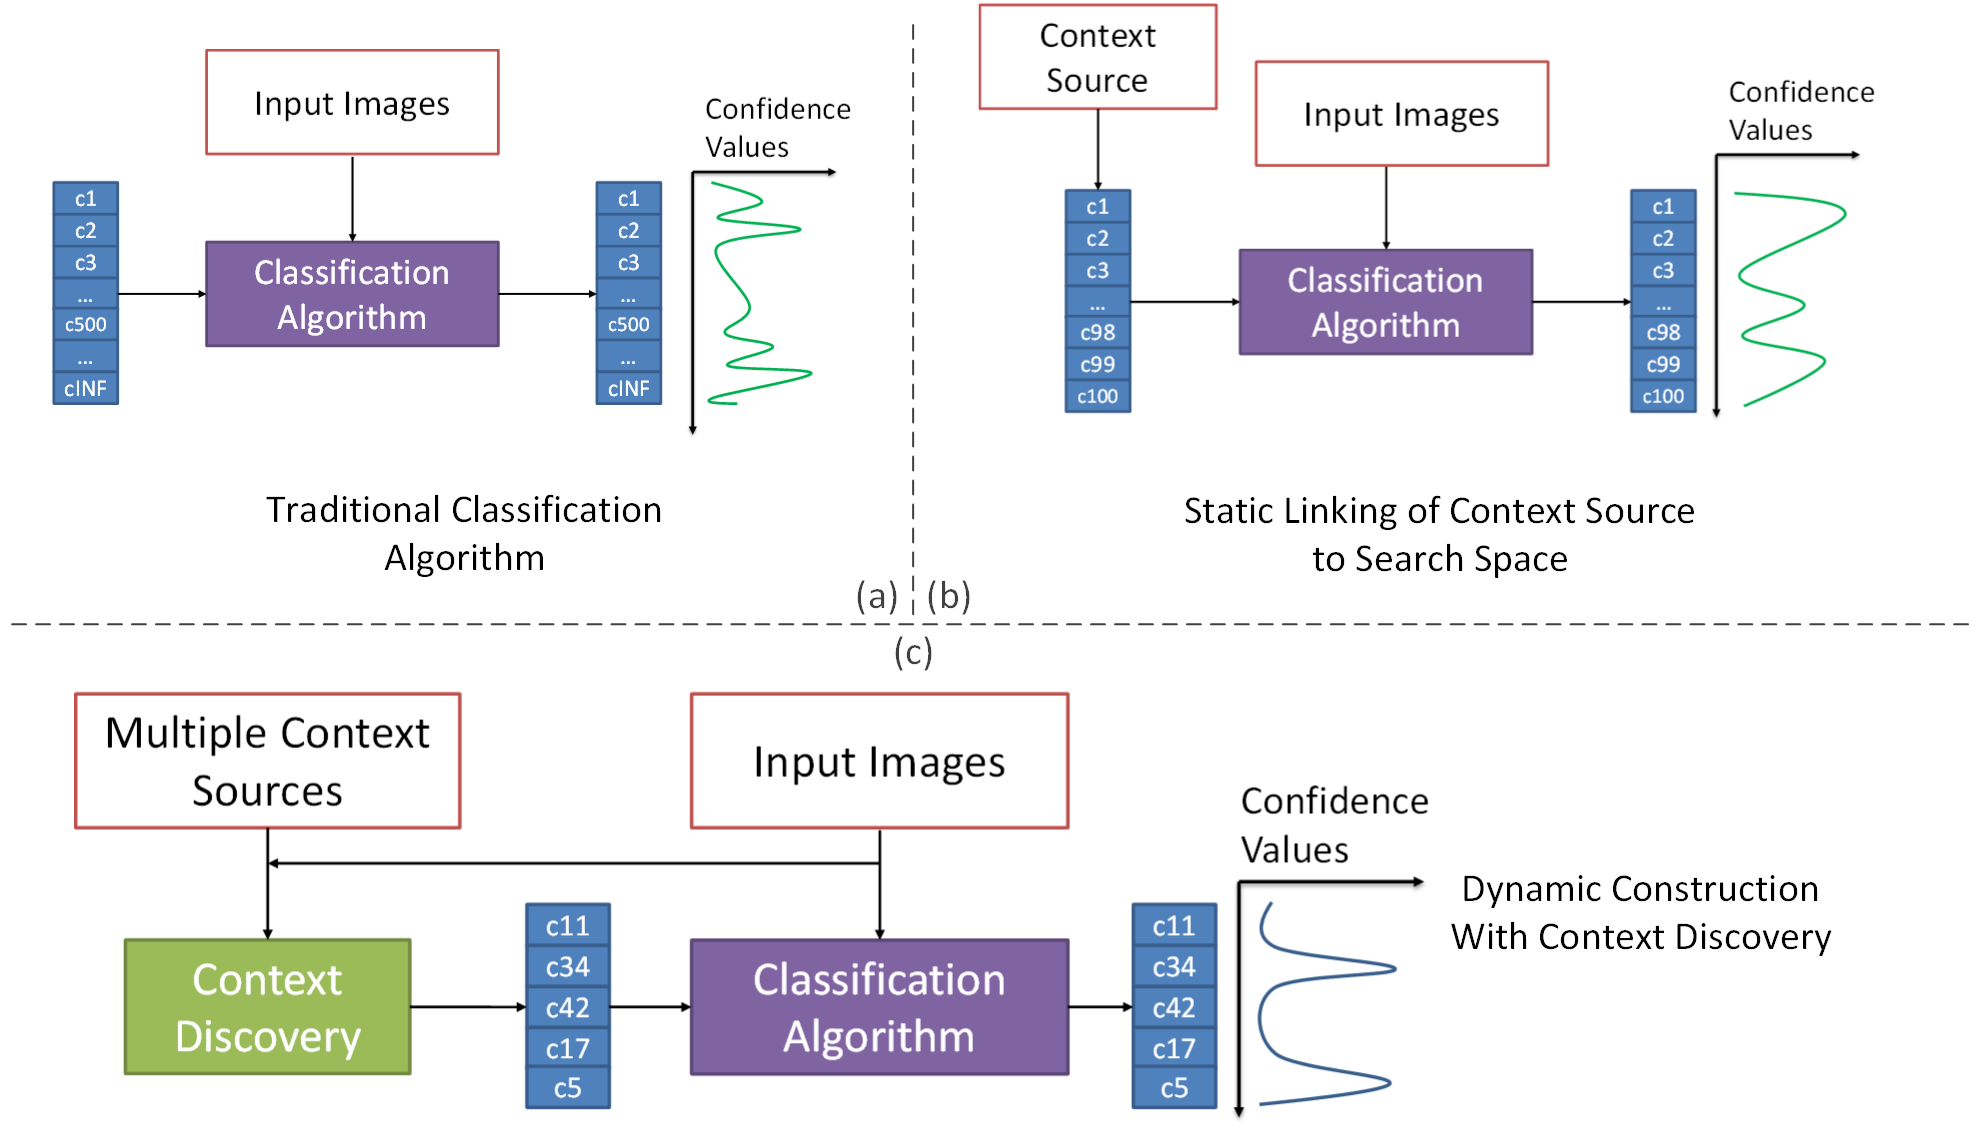
\includegraphics[width=0.95\textwidth]{media/with-without-cuenet-2.png}
\caption{The different approaches in search space construction for a multimedia annotation problem. A traditional classifier setup is shown in (a) where the search space candidates are manually specified. Context is used to generate large static search spaces in (b). The desired framework is shown in (c), which aims to produce small search spaces with many correct annotations.}
\label{fig:with-without-cuenet}
\end{figure}

With the popularity of global social networks and proliferation of mobile phones, information about people, their social connections and day-to-day activities are becoming available at a very large scale. The web provides an open platform for documenting many real world events like conferences, weather events and sports games. With such context sources, the search space construction is being delegated to one or a few sources \cite{henter2012tag, li2012fusing, naaman2005identity, o2009context,  stone2008autotagging} (figure \ref{fig:with-without-cuenet}(b)). These approaches rely on a single \textit{type} of context. For example, time and location information or social network information from Facebook to solve the face recognition problem. We refer to such a direct dependency between the search space and a data source as \textbf{static linking}. Although these systems are meritorious in their own right, they suffer from the following drawbacks: they do not employ multiple sources, and therefore the \textbf{relations} between them. By realizing that these sources are interconnected in their own way, we are able to treat the entire source topology as a network. Our intuition in this work is to navigate this network to progressively discover the search space for a given media annotation problem. Figure \ref{fig:with-without-cuenet}(c) shows how context discovery can provide substantially smaller search spaces for a set of images, which contain a large number of correct tags. A small search space with large number of true positives provides the ideal ground for a classification algorithm to exhibit superior performance.

We present the CueNet framework, which provides access to multiple data sources containing event, social, and geographical information through a unified query interface to extract information from them. CueNet encapsulates our \textbf{Context Discovery Algorithm}, which utilizes the query interface to discover the most relevant search space for a media annotation problem. To ensure a hands-on discussion, we show the use of context discovery in a real world application: face tagging in personal photos. As a case study, we will attempt to tag photos taken at conference events by different users. These photos could contain friends, colleagues, speakers giving very interesting talks, or newly found acquaintances (who are not yet connected to the user through any social network). This makes the conference photos particularly interesting because no single source can provide all the necessary information. It emphasizes the need to utilize multiple sources in a meaningful way.

\begin{figure}[t]
\centering
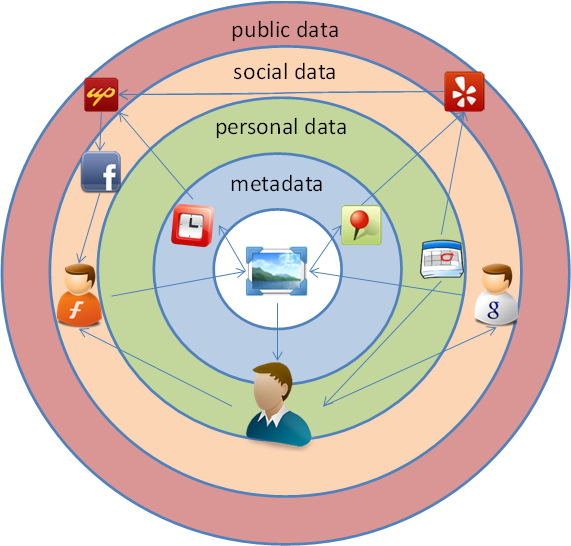
\includegraphics[width=0.65\textwidth]{media/prog-discovery.png}
\caption{Navigation of a discovery algorithm between various data sources.}
\label{fig:prog-discovery}
\end{figure}

Here is an \textbf{example} to illustrate CueNet's discovery process. Let's suppose that Joe takes a photo with a camera that records time and GPS in the photo's EXIF header. Additionally, Joe has two friends. One with whom he interacts on Google+, and the other using Facebook. The framework checks if either of them have any interesting event information pertaining to this time and location. We find that the friend on Google+ left a calendar entry describing an event (a title, time interval and name of the place). The entry also marks Joe as a participant. In order to determine the category of the place, the framework uses Yelp.com with the name and GPS location to find whether it is a restaurant, sports stadium or an apartment complex. If the location of the event was a sports stadium, it navigates to upcoming.com to check what event was occurring here at this time. If a football game or a music concert was taking place at the stadium, we look at Facebook to see if the friend ``Likes" the sports team or music band. By traversing the different data sources in this fashion, the number of people, who could potentially appear in Joe's photograph, was incrementally built up, rather than simply reverting to everyone on his social network or people who could be in the area where the photograph was taken. We refer to such navigation between different data sources to identify relevant contextual information as \textbf{progressive discovery}. The salient feature of CueNet is to be able to progressively discover events, and their associated properties, from the different data sources and relate them to the photo capture event. We argue that given this structure and relations between the various events, CueNet can make assertions about the presence of a person in the photograph. Once candidates have been identified by CueNet, they are passed to the face tagging algorithm (like \cite{facever_pami2010}), which can perform very well as their search space is limited to two candidates.

Figure \ref{fig:cuenet-arch} shows the different components of the CueNet framework. The Ontological \textbf{Event Models} specify various event and entity classes, and the different relations between them. These declared types are used to define the \textbf{Data Sources} which provides access to different types of contextual data. The \textbf{Person Verification Tools} consist of a database of people, their profile information and photos containing these people. When this module is presented with a candidate and the input photograph, it compares the features extracted from the candidate's photos and the input photo to find the confidence threshold. In this section, we describe each module, and how the context discovery algorithm utilizes them to accomplish its task.

\begin{figure}[t]
\centering
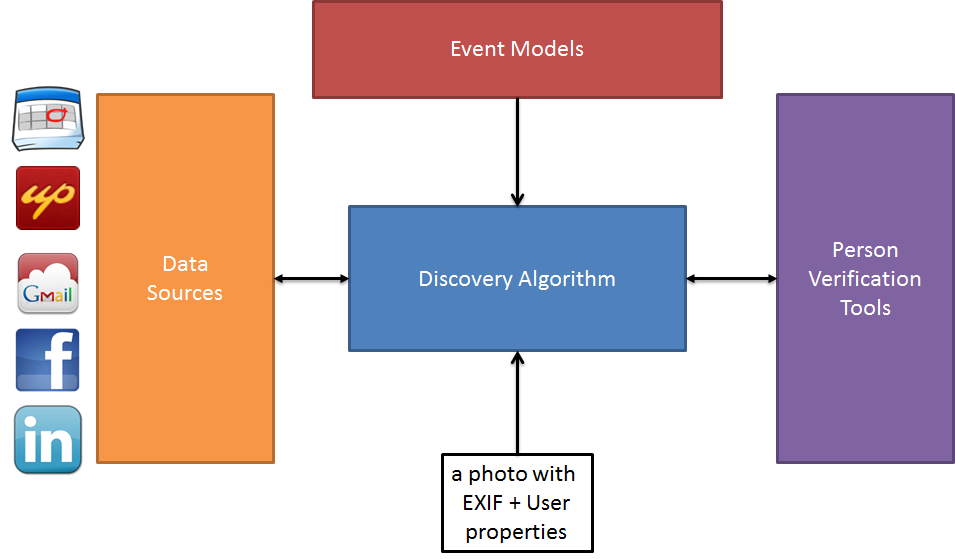
\includegraphics[width=0.9\textwidth]{media/cuenet-high-level-arch.png}
\caption{The Conceptual Architecture of CueNet.}
\label{fig:cuenet-arch}
\end{figure}

\section{General Approach}
What is our approach? How does context fit into? Describe a generic architecture of context discovery systems.

\section{Execution Trace}

\section{Event Model}
Our ontologies extend the E* model\cite{gupta2011managing} to specify relationships between events and entities. Specifically, we utilize the relationships ``\textbf{subevent-of}", which specifies event containment. An event $e1$ is a subevent-of of another event $e2$, if $e1$ occurs completely within the spatiotemporal bounds of $e2$. Additionally, we utilize the relations \textbf{occurs-during} and \textbf{occurs-at}, which specify the space and time properties of an event. Also, another important relation between entities and events is the ``\textbf{participant}" property, which allows us to describe which entity is participating in which event. It must be noted that participants of a subevent are also participants of the parent event. A participation relationship between an event and person instance asserts the presence of the person within the spatiotemporal region of the event. We argue that the reverse is also true, i.e., if a participant $P$ is present in $\mathcal{L}_P$ during the time $\mathcal{T}_P$ and an event $E$ occurs within the spatiotemporal region $<\mathcal{L}_E$, $\mathcal{T}_E>$, we say $P$ is a participant of $E$ if the event's spatiotemporal span contained that of the participant.
\begin{equation}
\label{eq:participation-region}
\begin{aligned}
\text{\texttt{participant}(E, P)} \iff (\mathcal{L}_P \sqsubset_L \mathcal{L}_E) \wedge (\mathcal{T}_P \sqsubset_T \mathcal{T}_E)
\end{aligned}
\end{equation}
The symbols $\sqsubset_L$ and $\sqsubset_T$ indicate spatial and temporal containment respectively. Please refer to \cite{gupta2011managing} for more details. In later sections, we refer to the location and time of the event, $\mathcal{L}_E$ and $\mathcal{T}_E$ as $E$.\textbf{occurs-at} and $E.$\textbf{occurs-during} respectively. 

\begin{figure*}[t]
\centering
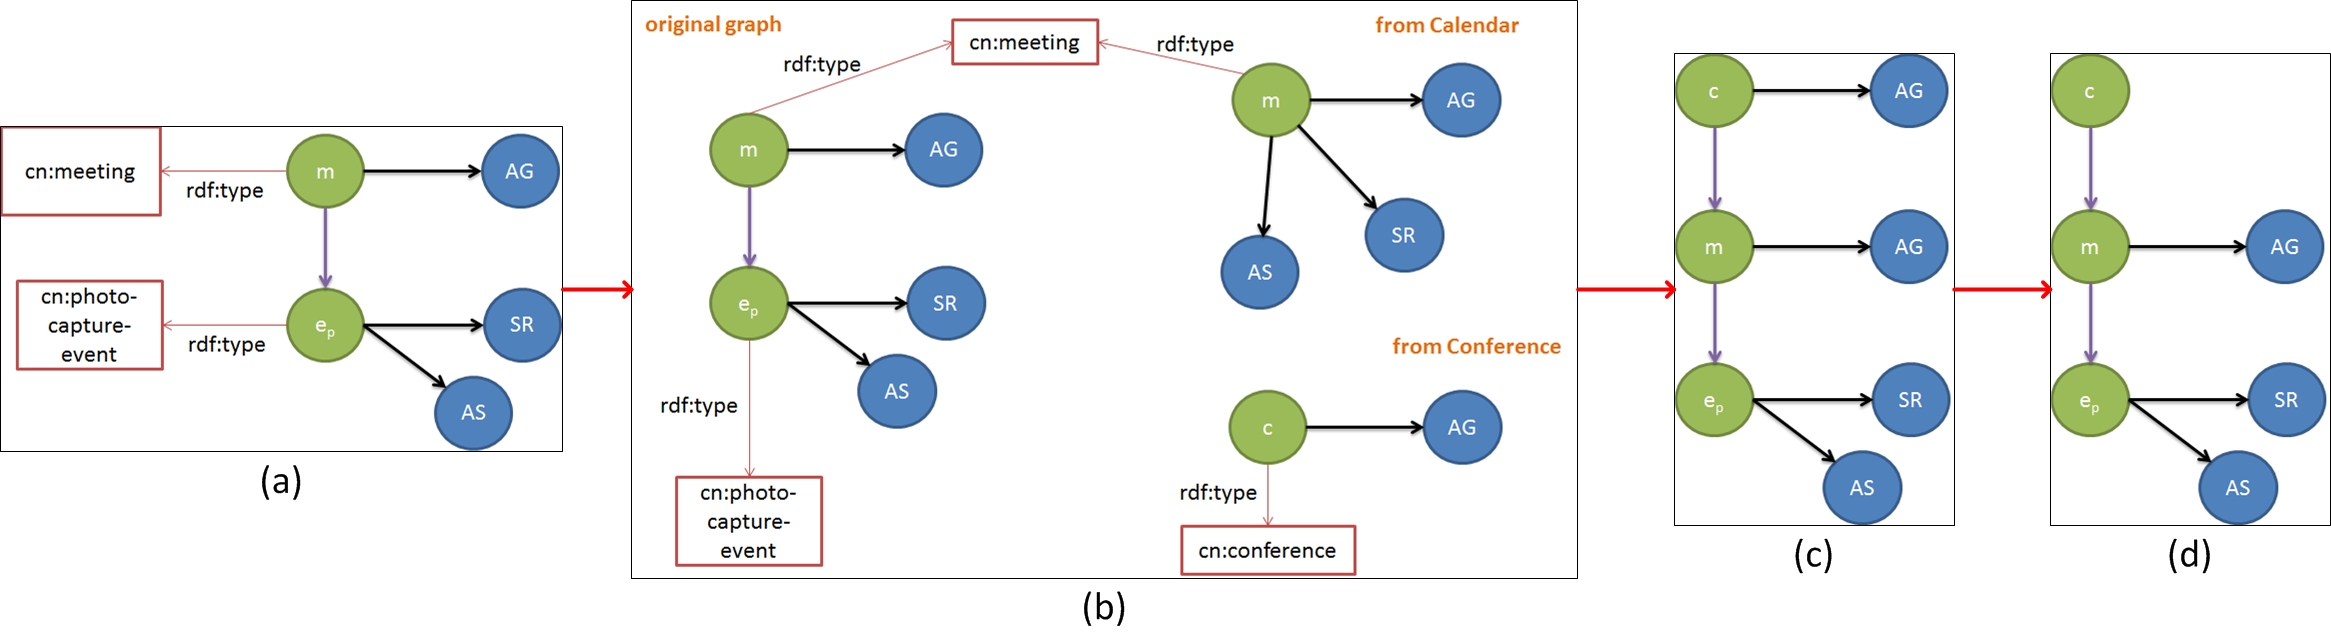
\includegraphics[width=\textwidth]{media/exec/exec-cycle-one-line.png}
\caption{The various stages in an iteration of algorithm \ref{alg:cx-alg}.}
\label{fig:exec-cycle}
\end{figure*}

\section{Data Sources}
\label{sec:data-sources}
The ontology makes available a vocabulary of classes and properties. Using this vocabulary, we can now declaratively specify the schema of each source. With these schema descriptions, CueNet can infer what data source can provide what type of data instances. For example, the framework can distinguish between a source which describes conferences and another which is a social network. We use a LISP like syntax to allow developers of the system to specify these declarations. The example below describes a source containing conference information.

\begin{verbatim}
(:source conferences
   (:attrs url name time location title)
   (:rel conf type-of conference)
   (:rel time type-of time-interval)
   (:rel loc type-of location)
   (:rel attendee type-of person)
   (:rel attendee participant-in conf)
   (:rel conf occurs-at loc)
   (:rel conf occurs-during time)
   (:axioms
      (:map time time)
      (:map loc location)
      (:map conf.title ltitle)
      (:map conf.url url)
      (:map attendee.name name)))
\end{verbatim}

% The above source declaration consists of a s-expression, where the source keyword indicates a unique name for the source. The \texttt{attrs} keyword is used to list the attributes of this source. The \texttt{rel} keyword constructs the instances conf, time, loc, attendee which are of conference, time-interval, location and person class types respectively, and relates them with relations specified in the ontology. Finally, the mapping \texttt{axioms} are used to map nodes in the relationship graph constructed above to attributes of the data source. For example, the first axiom (specified using the map keyword) maps the time node to the time attribute. 

A source declaration comprises of a single nested s-expression. We will refer to the first symbol in each expression as a keyword, and the following symbols as operands. This above declaration uses five keywords (\texttt{source}, \texttt{attrs}, \texttt{rel}, \texttt{axioms}, \texttt{map}).  The \texttt{source} keyword is the root operator, and declares a unique name of the data source. The source mapper can be queried for finding accessors using this name. The \texttt{attrs} keyword is used to list the attributes of this source. Currently we assume a tuple based representation, and each operand in the attrs expression maps to an element in the tuple. The \texttt{rel} keyword allows construction of a relationship graph where the nodes are instances of ontology concepts. And edges are the relationships described by this particular source. In the above example, we construct individuals \textit{conf}, \textit{time}, \textit{loc} and \textit{attendee} who are instances of the \textit{conference}, \textbf{time-interval}, \textbf{location} and \textbf{person} class respectively. We further say that attendee is a \textbf{\textit{participant of}} the conference, which \textbf{\textit{occurs-at}} location loc and \textbf{\textit{occurs-during}} the interval time. Finally, the \texttt{mapping axioms} are used to map nodes in the relationship graph to attributes of the data source. For example, the first axiom (specified using the map keyword) maps the time node to the time attribute. The third map expression creates a literal called title, and associates it to the conference node, whose value comes from the ltitle attribute of the conference data source.

Formally, we represent the given ontology as $O$. The various classes and properties in $O$ are represented by $C^O$ and $P^O$ respectively. Since our upper ontology consists of DOLCE and E*, we assume the inclusion of the classes \texttt{Endurant}, \texttt{Perdurant}, \texttt{Event} and \texttt{Person} in $C^O$. Each source $S$ consists of three parts, a relation graph $G^S(V^S, E^S)$ where the nodes $V^S \in C^O$, specify the various ``things'' described by the source. The edges $E^S \in P^O$ specify the relations among the nodes. Any graph retrieved from such a source is an instance of the relation graph, $G^S$. Further, the tuple $A^S_T$ consists of the attributes of the data source. Finally, the mapping $M^S: \{G^S \rightarrow A^S_T\}$ specifies how to map different nodes in the relation graph to the different attributes of the native data source.

\section{Conditions for Discovery}
CueNet is entirely based on reasoning in the event and entity (i.e., person) domain, and the relationships between them. These relationships include participation (event-entity relation), social relations (entity-entity relation) and subevent relation (event-event). For the sake of simplicity, we restrict our discussions to events whose spatiotemporal spans either completely overlap or do not intersect at all. We do not consider events which partially overlap. In order to develop the necessary conditions for context discovery, we consider the following two axioms:

\textbf{Entity Existence Axiom}: Entities can be present in one place at a time only. The entity cannot exist outside a spatiotemporal boundary containing it.

\textbf{Participation Semantics Axiom}: If an entity is participating in two events at the same time, then one is the subevent of the other. 

% Before we provide an overview of the discovery algorithm, we must make a note of set of conditions required for its correct execution. 

Given, the ontology $O$, we can construct event instance graph $G^I(V^I, E^I)$, whose nodes are instances of classes in $C^O$ and edges are instances of the properties in $P^O$. The context discovery algorithm relies on the notion that given an instance graph, \textit{queries} to the different sources can be automatically constructed. A query is a set of predicates, with one or more unknown variables. For the instance graph $G^I (V^I, E^I)$, we construct a query $Q(D, U)$ where $D$ is a set of predicates, and $U$ is a set of unknown variables.

\textbf{Query Construction Condition:} Given an instance graph $G^I (V^I, E^I)$ and ontology $O(C^O, P^O)$, a query $Q(D, U)$ can be constructed, such that $D$ is a set of predicates which represent a subset of relationships specified in $G^I$. In other words, $D$ is a subgraph induced by $G^I$. $U$ is a class, which has a relationship $r \in P^O$, with a node $n \in D$. Essentially, the ontology must prescribe a relation between some node $n$ through the relationship $r$. In our case, the relation $r$ will be either a \textbf{participant} or \textbf{subevent} relation. If the relationship with the instances does not violate any object property assertions specified in the ontology, we can create the query $Q(D, U)$.

\textbf{Identity Condition:} Given an instance graph $G^I(V^I, E^I)$, and a result graph $G^R(V^R, E^R)$ obtained from querying a source, we can merge two events only if they are identical. Two nodes $v^I_i \in V^I$ and $v^R_r \in V^R$ are identical if they meet the following two conditions \textbf{(i)} Both $v^I_i$ and $v^R_r$ are of the same class type, and \textbf{(ii)} Both $v^I_i$ and $v^R_r$ have exactly overlapping spatiotemporal spans, indicated by the $=_L$ and $=_T$. Mathematically, we write: 
\begin{equation}
\label{eq:identity}
\begin{aligned}
v^I_i = v^R_r \iff (v^I_i.\text{\textbf{type-of}} = v^R_r.\text{\textbf{type-of}}) \wedge \\ 
(v^I_i.\text{\textbf{occurs-at}} =_L v^R_r.\text{\textbf{occurs-at}}) \wedge \\
(v^I_i.\text{\textbf{occurs-during}} =_T v^R_r.\text{\textbf{occurs-during}})
\end{aligned}
\end{equation}
\textbf{Subevent Condition:} Given an instance graph $G^I(V^I, E^I)$, and a result graph $G^R(V^R, E^R)$ obtained from querying a source, we can construct a subevent edge between two nodes $v^I_i \in V^I$ and $v^R_r \in V^R$, if one is spatiotemporally contained within the other, and has at least one common \texttt{Endurant}.
\begin{equation}
\label{eq:sube-st-containment}
\begin{aligned}
   v^I_i \sqsubset_L v^R_r,\\
   v^I_i \sqsubset_T v^R_r
\end{aligned}
\end{equation}
\begin{equation}
\label{eq:sube-entity-containment}
\begin{aligned}
   v^I_i.\text{\textbf{Endurants}} \cap v^R_r.\text{\textbf{Endurants}} \neq \{\phi\}\\
\end{aligned}
\end{equation}
Here $v^I_i.$\textbf{Endurants} is defined as a set $\{w | w \in V^I_i \wedge w.$type-of$ = $Endurant$\}$. If equation \eqref{eq:sube-entity-containment} does not hold, we say that $v^I_i$ and $v^R_r$ co-occur.

\textbf{Merging Event Graphs}: Given the above conditions, we can now describe an important building block for the context discovery algorithm: the steps needed to merge two event graphs. An example for this is shown in figure \ref{fig:exec-cycle}(b-d). Given the event graph consisting of the photo capture event on the left of (b) and a meeting event $m$ and conference event $c$, containing their respective participants. In this example, the meeting event graph, $m$ is semantically equivalent to the original graph. But the conference event, $c$ is telling that the person $AG$ is also participating in a conference at the time the photo was taken. The result of merging is shown in (d). An event graph merge consists of two steps. The first is a \texttt{subevent hierarchy join}, and the second is a \texttt{prune-up} step. 

Given an original graph, $O_m$, and a new graph $N_m$, the join function works as follows: All nodes in $N_m$ are checked against all nodes in $O_m$ to find identical counterparts. For entities, the identity is verified through an identifier, and for events, equation \eqref{eq:identity} is used. Because of the entity existence and participation semantics axioms, all events which contain a common participant are connected to their respective super event using the subevent relation (equations \eqref{eq:sube-st-containment} and \eqref{eq:sube-entity-containment} must be satisfied by the events). Also, if two events have no common participant, then they can be still be related with the subevent edge, if the event model says it is possible. For example, if in a conference event model, keynotes, lunches and banquets are declared as known subevents of an event. Then every keynote event, or banquet event to be merged into an event graph is made a subevent of the conference event, if the equation \eqref{eq:sube-st-containment} holds between the respective events. 

It must be noted that node $AG$ occurs twice in graph (c). In order to correct this, we use the participation semantics axiom. We traverse the final event graph from the leaves to the root events, and remove every person node if it appears in a subevent. This is the \texttt{prune-up} step. Using these formalisms, we now look at the working of the context discovery algorithm. 

\restylealgo{ruled}
\SetAlgoSkip{}
\begin{algorithm}[t]
\dontprintsemicolon 
\KwData{A photograph H, with a set of detected faces F. Voting threshold, T. The owner O of the photo.}
\KwResult{For each face f $\in$ F, a set of atmost $k$ person tags.}
\Begin{
  
  $ $\;
  function discover(): \{ \;
  \Indp while (\texttt{DQ} is not empty): \{ \;
  \Indp \texttt{node} = \texttt{DQ}.deque() \;
  \texttt{results} = query (\texttt{node}) \;
  \texttt{E} $\leftarrow$ merge (\texttt{E}, \texttt{results}) \;
  if (termination\_check()): \;
  \Indp \textbf{return} prepare\_results(); \;
  \Indm
  \Indm
  \} \;
  reconstruct \texttt{DQ} $\leftarrow$ \texttt{E} \;
  discover() \;
  \Indm
  \}\;
  
  $ $\;
  
  function merge(\texttt{O}, \texttt{N}): \{ \;
    \Indp 
    remove\_duplicates() \;
    \texttt{M} $\leftarrow$ subevent\_hierarchy\_join(\texttt{O}, \texttt{N}) \;
    prune\_up(\texttt{M}) \;
    if (less than \texttt{T} new candidates were discovered): \; {
    \Indp
  	    push\_down(\texttt{M}) \;
  	\Indm
    } else: \; 
    \Indp
	    vote\_and\_verify(\texttt{M}) \;
  	\Indm
 	return \texttt{M}; \;
  \Indm
  \} 
  
  $ $ \;
  \texttt{E} $\leftarrow$ construct event graph with \texttt{H} and \texttt{O} \;
  construct discoverable nodes queue, \texttt{DQ} $\leftarrow$ \texttt{E} \;
  \textbf{return} discover() \;
  
}
\caption{The Context Discovery Algorithm}
\label{alg:cx-alg}
\end{algorithm}

\subsection{Context Discovery Algorithm}
\label{sec:discovery-algorithm}
Algorithm \ref{alg:cx-alg} below outlines the tail recursive discovery algorithm. The input to the algorithm is a photo (with EXIF tags) and an associated owner (the user). It must be noted that by seeding the graph with owner information, we bias the discovery towards his/her personal information. An event instance graph is created where each photo is modeled as a photo capture event. Each event and entity is a node in the instance graph. Each event is associated with time and space attributes. All relationships are edges in this graph. All EXIF tags are literals, related to the photo with data property edges. Figure \ref{fig:exec-cycle} graphically shows the main stages in a single iteration of the algorithm.

The event graph is traversed to produce a queue of entity and event nodes, which we shall refer to as DQ (discovery queue). The algorithm consists of two primary functions: \textbf{discover} and \textbf{merge}. The discover function is tail recursive, invoking itself until a termination condition is reached (when at most $k$ tags are obtained for all faces or no new data is obtained from all data sources for all generated queries). The behavior of the query function depends on the type of the node. If the node is an event instance, the function consults the ontology to find any known sub-events, and queries data sources to find all these subevents, its properties and participants of the input event node. On the other hand, if it is an entity instance, the function issues a query to find all the events it is participating in. 

Results from data source wrappers are returned in the form of event graphs. These event graphs are merged into the original event graph by taking the following steps. First, it identifies \textbf{duplicate} events using the conditions mentioned above. Second, it identifies subevent hierarchies using the graph merge conditions described above, and performs a \textbf{subevent hierarchy join}. Third, the function \textbf{prune-up} removes entities from an event when its subevent also lists it as a participant node. Fourth, \textbf{push-down} is the face verification step if the number of entities in the parents of the photo-capture events is small (less than $T$). Push down will try to verify if any of the newly discovered entities are present in the photo and if they are (if the tagging confidence is higher than the given threshold), the entities are removed from the super event, and linked to the photo capture event as its participant. On the other hand, if this number is larger than T, the algorithm initiates the \textbf{vote-and-verify} method, which ranks all the candidates based on social relationships with people already identified in the photo. For example, if a candidate is related to two persons present in the photo through some social networks, then its score is 2. Ranking is done by simply sorting the candidate list by descending order of score. The face verification runs only on the top ranked $T$ candidates. If there are still untagged faces after the termination of the algorithm, we vote over all the remaining people, and return the ranked list for each untagged face.

Figure \ref{fig:exec-cycle} shows the various stages in the algorithm graphically. (a) shows an example event graph describing a photo taken at a meeting. The meeting consists of three participants AG, SR and AS. The photo contains SR and AS. (b) shows two events returned from the data sources. One is a meeting event which is semantically identical to the input. The other is a conference event with AG. (c) shows the result of merging these graphs. (d) The \texttt{prune-up} function removes the duplicate reference to AG. \underline{A live visualization of these steps for different photos can be found at \href{http://cuenet.site44.com/}{http://cuenet.site44.com}}.

\section{Implementation}
